\documentclass[11pt,a4paper,twoside]{article}
\usepackage[includeheadfoot, left=3cm, right=2cm, top=2.5cm, bottom=2.5cm, headheight=19.3pt]{geometry}

\usepackage[polish]{babel}
\usepackage[T1]{fontenc}
\usepackage[utf8]{inputenc}
\usepackage[scaled]{helvet}
\renewcommand\familydefault{\sfdefault} 

\let\lll=\relax
\usepackage{amsmath}
\usepackage{amsfonts}
\usepackage{amssymb}
\usepackage{bm}

\usepackage{url}
\usepackage{pdfpages}
\usepackage[bookmarks, pagebackref]{hyperref}
\usepackage[none]{hyphenat}
\usepackage{graphicx}
\usepackage{color}
\usepackage{array}
\usepackage{subfiles}
\usepackage{etoolbox, fancyhdr, xcolor}
\usepackage[hang, flushmargin]{footmisc}
\usepackage{setspace}
\usepackage{ragged2e}
%\usepackage{MnSymbol}
\usepackage[nottoc]{tocbibind}
\usepackage{titlesec}
\urlstyle{rm}
\usepackage[ampersand]{easylist}
\usepackage{enumitem}
\usepackage{epsfig}
\usepackage{float}
\usepackage[font={up, footnotesize}, labelfont=bf, singlelinecheck=off, format=hang]{caption}
\usepackage{caption}
\usepackage{subcaption}
\usepackage{listings}
\lstset{language=C++, rulecolor=\color{sapphire}, framerule=1.5pt} % you can change language of your code
\usepackage{colortbl}
\usepackage{tabu}
\usepackage{makecell}
%\usepackage{boldline}
\setlength{\arrayrulewidth}{1pt}
\captionsetup[table]{name=Table}

\usepackage{lipsum} % for testing purposes

\definecolor{sapphire}{RGB}{120,150,207}
\definecolor{grafit}{RGB}{60,60,60}

% pdf output setup
\hypersetup{
	unicode,
	pdftoolbar,
	pdfmenubar,
	pdffitwindow,
	pdfstartview = {FitH},
	pdftitle = {Praca Inżynierska}, 
	pdfauthor = {Imię i nazwisko},
	pdfnewwindow,
	colorlinks,
	linktoc = page,
	% use color sapphire or grafit
	linkcolor = sapphire,
	citecolor = sapphire,
	filecolor = sapphire,
	urlcolor = black
}


\newcommand{\itemi}[1][sapphire]{\item[\color{#1} $\filledsquare$]}
\newcommand{\itemii}[1][sapphire]{\item[\color{#1} $\square$]}
\newcommand{\itemiii}[1][sapphire]{\item[\color{#1} $\bullet$]}

\ListProperties(Hide=100, Progressive=1cm, Style=\color{sapphire}, Style**=\color{black}, Style*=$\square$ ,Style2*=$\bullet$)


\newcommand{\headrulecolor}[1]{\patchcmd{\headrule}{\hrule}{\color{#1}\hrule}{}{}}
\newcommand{\footrulecolor}[1]{\patchcmd{\footrule}{\hrule}{\color{#1}\hrule}{}{}}


\newcommand{\infostyle}[1]
{
	\fancyhf{}
	\fancyhead[LO]{\Large{\textbf{#1}}}

	\renewcommand{\headrulewidth}{1.5pt}
	\headrulecolor{sapphire}
	\justify
	\pagestyle{fancy}
}


\newcommand{\thesisstyle}
{
	\fancyhf{}
	\fancyhead[RO,LE]{\Large{\textbf{\rightmark}}}
	\fancyfoot[LE,RO]{\thepage}

	\renewcommand{\headrulewidth}{1.5pt}
	\renewcommand{\footrulewidth}{1.5pt}
	\headrulecolor{sapphire}
	\footrulecolor{sapphire}
	\justify
	\pagestyle{fancy}
}


\newcommand{\fancyfootnotetext}[2]
{
	\fancypagestyle{footnotes}
	{
    	\fancyfoot[LO,RE]{\parbox{15cm}{\footnotemark[#1]\footnotesize #2}}
	}
	\thispagestyle{footnotes}
}


\newcommand{\fancyfootnotetexts}[4]
{
	\fancypagestyle{footnotes}
	{
    	\fancyfoot[LO,RE]{\parbox{15cm}{\footnotemark[#1]\footnotesize #2 \\ \footnotemark[#3]\footnotesize #4}}
	}
	\thispagestyle{footnotes}
}


\newcommand{\fancyfootnotetextss}[6]
{
	\fancypagestyle{footnotes}
	{
    	\fancyfoot[LO,RE]{\parbox{15cm}{\footnotemark[#1]\footnotesize #2 \\ \footnotemark[#3]\footnotesize #4 \\ \footnotemark[#5]\footnotesize #6 \\}}
	}
	\thispagestyle{footnotes}
}


\titlespacing\section{0pt}{15pt}{10pt} 
\titlespacing\subsection{0pt}{15pt}{10pt} 
\titlespacing\subsubsection{0pt}{15pt}{10pt} 

\setstretch{1.15}
\setlength{\parindent}{0.5cm} 
\setlength{\parskip}{0cm} 

\frenchspacing
\sloppy

\author{} 
\title{} 
\date{}
\graphicspath{{images/}}

\begin{document}


\includepdf[pages={-}]{preamble/begining.pdf}
\tableofcontents
\thispagestyle{empty}
\thesisstyle
\newpage 

\section[Wstęp]{Wstęp}
\lipsum[1-5]

\section[Część analityczna]{Część analityczna/Problematyka pracy}
\subsection{Przegląd literatury}
\lipsum[1-3]
\subsection{Jak się robi cośtam}
\lipsum[1-3]
\subsection{Jak się robi cośtam jeszcze innego}
\lipsum[1-2]

\newpage
\section[Część syntetyczna]{Część syntetyczna/Wybór metod}
\subsection{Dlaczego wybrałem/am tą metodę}
\lipsum[1-3]
\subsection{Dlaczego wybrałem/am tamtą metodę}
\lipsum[1-3]

\newpage
\section[Część weryfikacyjna]{Część weryfikacyjna/Wyniki eksperymentów/Wyniki symulacji}
\subsection{Badanie jednej rzeczy}
\lipsum[1-3]
\subsection{Badanie tej samej rzeczy, ale inaczej}
\lipsum[1-3]
\subsection{Badanie tego, ale jeszcze inaczej}
\lipsum[1-3]

\section[Zakończenie]{Zakończenie/Wnioski/Podsumowanie}
\lipsum[1-8]

\newpage
\section[Przykłady]{Przykłady rysunków, tabel itp.}
\subsection{Listowanie}
Listuje się w sposób następujący:
\begin{itemize}
	\itemi pierwszy poziom listy - element pierwszy,
	\itemi pierwszy poziom listy - element drugi,
	\begin{itemize}
		\itemii drugi poziom listy - element pierwszy,
		\itemii drugi poziom listy - element drugi,
		\itemii drugi poziom listy - element trzeci,
		\begin{itemize}
			\itemiii trzeci (ostatni) poziom listy - element pierwszy,
			\itemiii trzeci (ostatni) poziom listy - element drugi,
			\itemiii trzeci (ostatni) poziom listy - element trzeci,
		\end{itemize}
		\itemii drugi poziom listy - element czwarty,
		\end{itemize}
	\itemi pierwszy poziom listy - element trzeci,
	\itemi pierwszy poziom listy - element czwarty.
\end{itemize}

\subsection{Cytowania i przypisy}
This document is an example of BibTeX using in bibliography management. Three items 
are cited: \textit{The \LaTeX\ Companion} book \cite{latexcompanion}, the Einstein
journal paper \cite{einstein}, and the Donald Knuth's website \cite{knuthwebsite}. 
The \LaTeX\ related items are \cite{latexcompanion,knuthwebsite}.\footnotemark[1]

\fancyfootnotetextss{1}{Źródło: \url{https://www.sharelatex.com/learn/Bibliography_management_with_bibtex}}{2}{Niestety nie ma automatycznej numeracji przypisów.}{3}{Ich liczba na stronie ograniczona jest do trzech (jednak można to rozszerzyć)}

\subsection{Wzory}
Równania reakcji-dyfuzji
\begin{align}
	\begin{cases}
		\frac{\partial}{\partial t} u(\bm{x},t) = f(u,v) + D_{act}\nabla^{2} u(\bm{x},t) \\
		\frac{\partial}{\partial t} v(\bm{x},t) = g(u,v) + D_{inh}\nabla^{2} v(\bm{x},t)
	\end{cases}
\end{align}
gdzie: \\ 
\indent $u(\bm{x},t)$ -- koncentracja aktywatora, \\
\indent $v(\bm{x},t)$ -- koncentracja inhibitora, \\
\indent $D_{act}$ -- stała dyfuzji aktywatora, \\
\indent $D_{inh}$ -- stała dyfuzji inhibitora. \\

\newpage
\subsection{Obrazki}

Przykładowe, niezwiązane ze sobą, obrazki:
\begin{figure}[H]
	\centering
	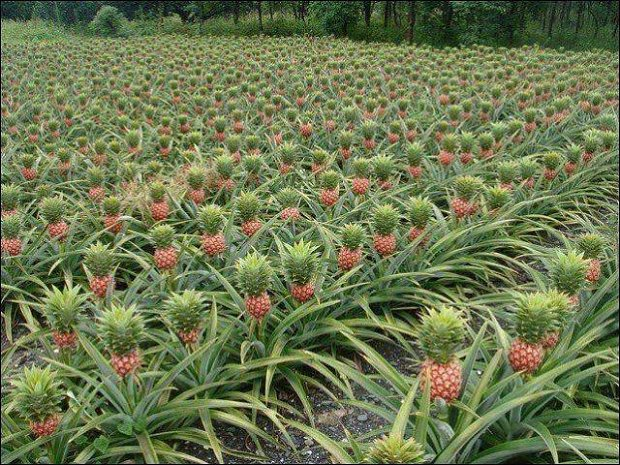
\includegraphics[width=0.65\textwidth]{pole_ananasowe.jpg}
    \captionsetup{justification=raggedleft, font={it, footnotesize}}
    \caption*{\url{http://vader.joemonster.org/upload/qpm/l_13484426e12385bananasplantage.jpg}} 
    \captionsetup{justification=justified, font={up, footnotesize}}
    \caption{Tak wygląda ananasowe pole. Przykład wklejania grafiki rastrowej.}
    \label{rys1}
\end{figure}

\begin{figure}[H]
	\centering
	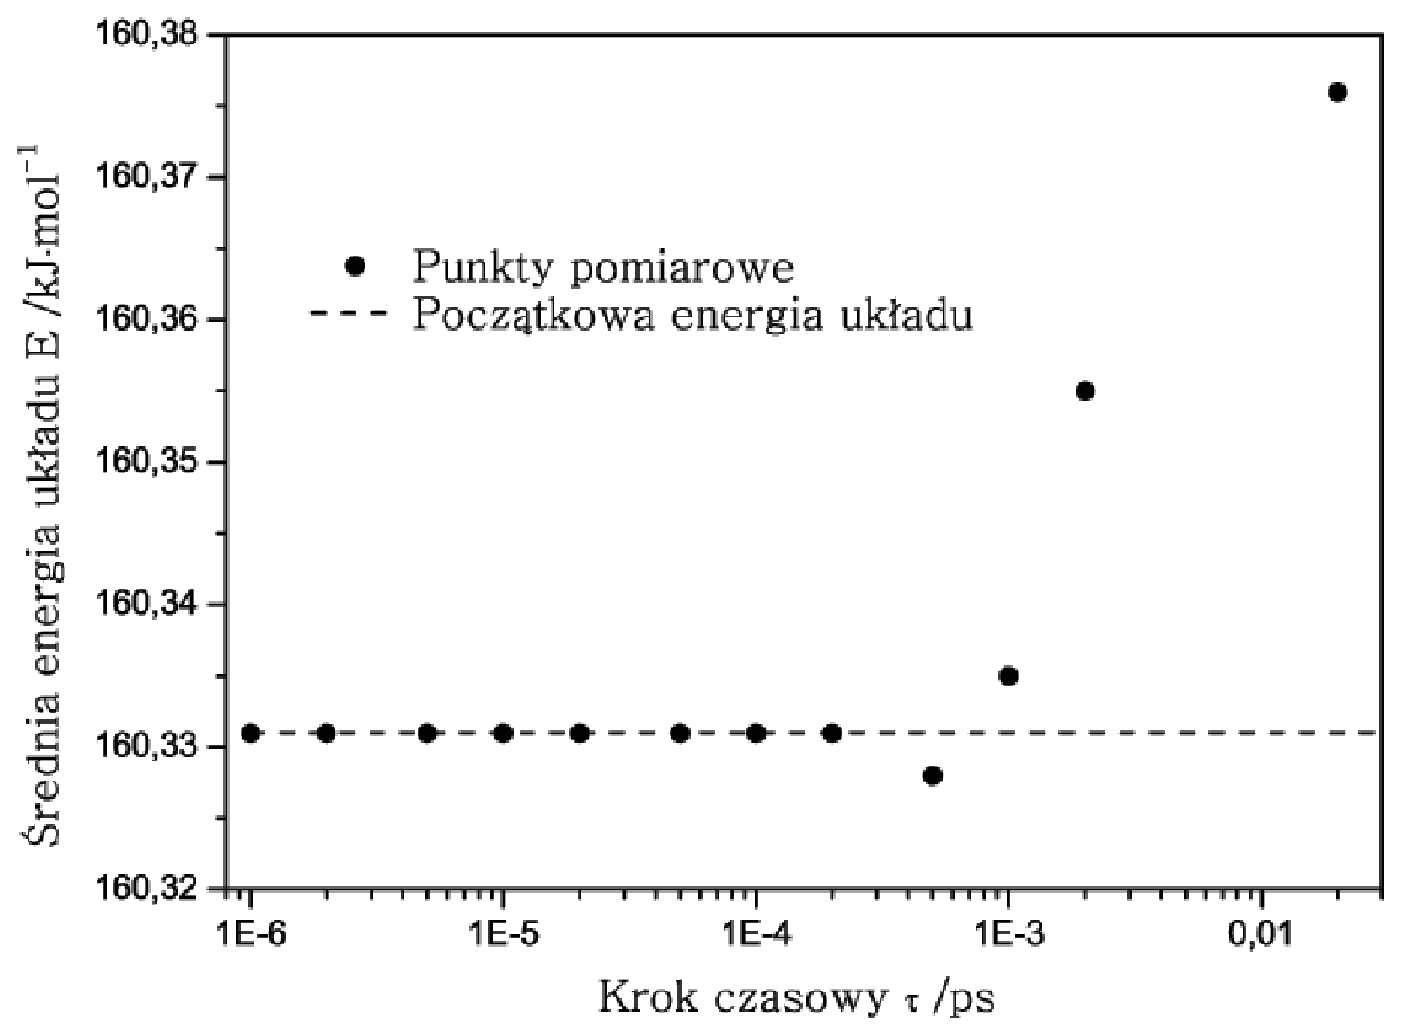
\includegraphics[width=0.65\textwidth]{krok_czasowy}
    \captionsetup{justification=justified}
    \caption{Test algorytmu -- średnia energia w funkcji kroku czasowego. Przykład wklejania grafiki wektorowej. Brak źródła świadczy o własnoręcznym wykonaniu obrazka.}
    \label{rys2}
\end{figure}

\newpage
Czy są osoby, które nie wiedzą co to są szachy? Zapewne nie, jednak mimo wszystko, krótkie przypomnienie:
\begin{figure}[H]
	\begin{subfigure}{0.40\textwidth}
		\centering
 		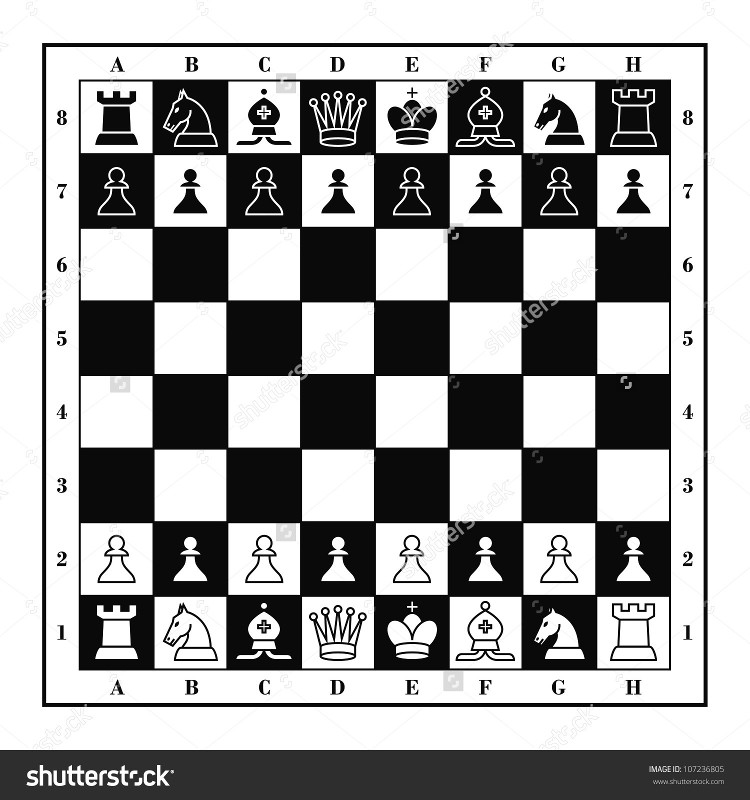
\includegraphics[width=\textwidth]{szachownica.jpg}
 		\captionsetup{font={up, footnotesize}}
    	\caption{Początkowe położenie figur.}
 		\label{rys3}
	\end{subfigure}
	\hfill
	\begin{subfigure}{0.40\textwidth}
		\centering
		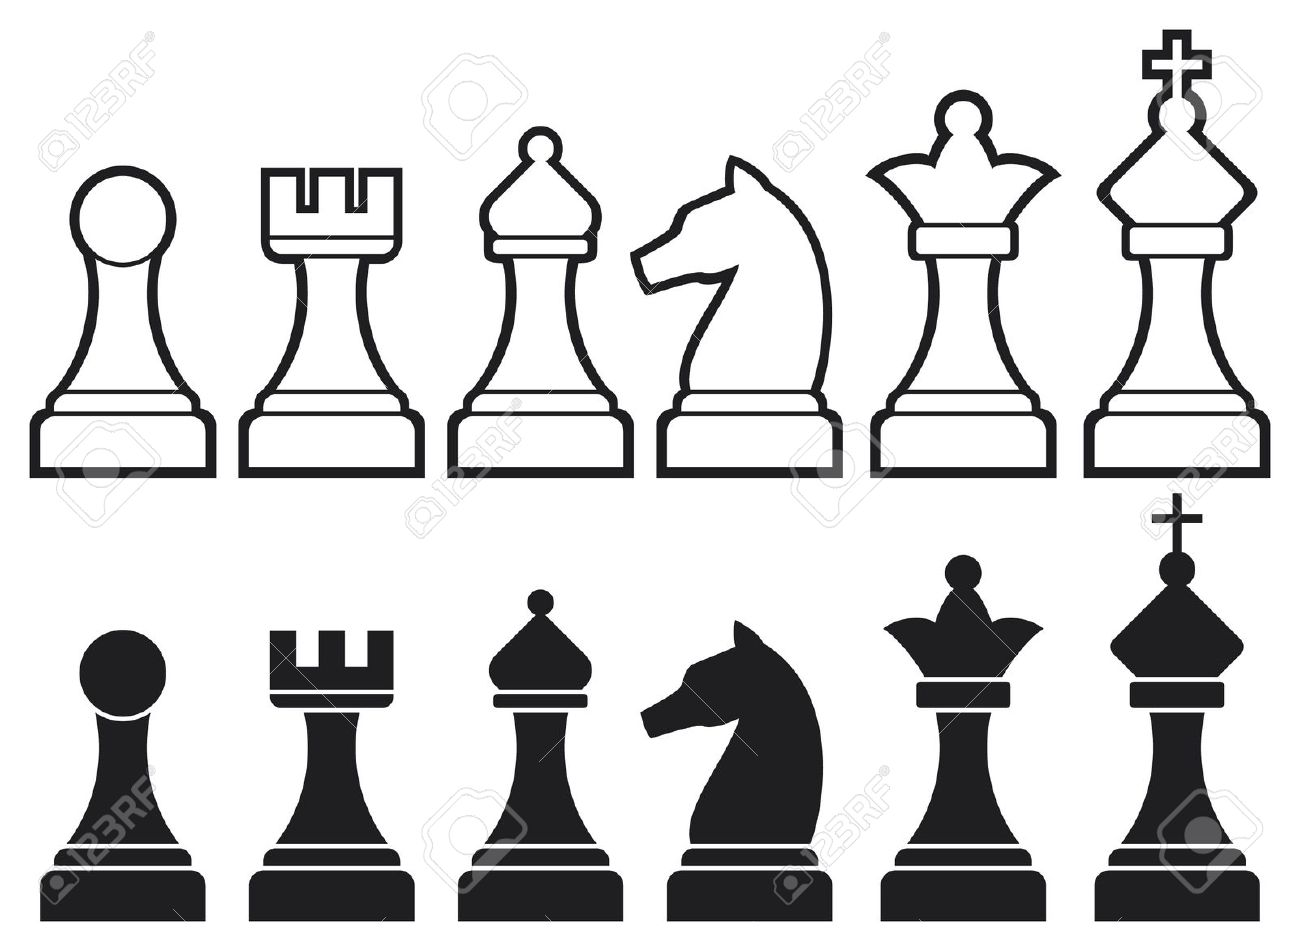
\includegraphics[width=\textwidth]{figury_szachowe.jpg}
		\captionsetup{font={up, footnotesize}}
    	\caption{Figury występujące w grze.}
		\label{rys4}
	\end{subfigure}
	\vskip\baselineskip
	\begin{subfigure}{0.40\textwidth}
		\centering
 		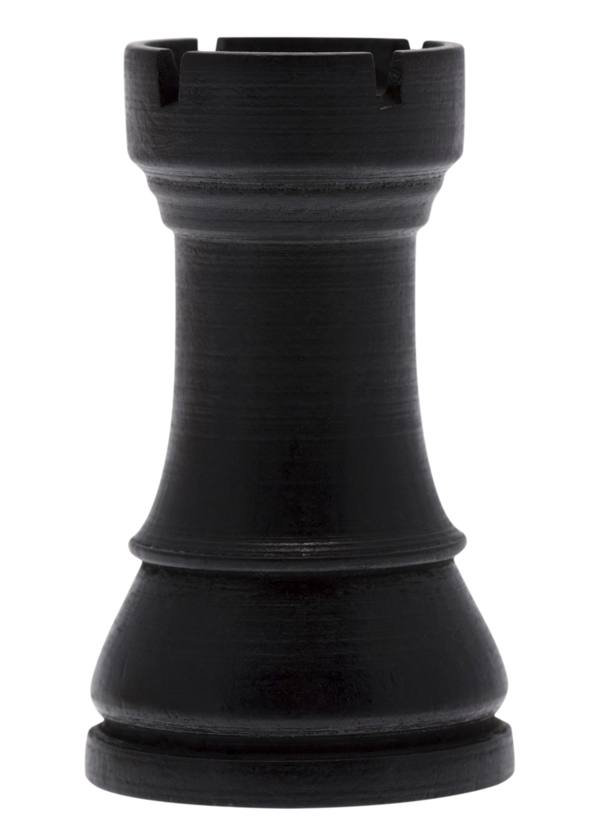
\includegraphics[width=\textwidth]{wieza.jpg}
 		\captionsetup{font={up, footnotesize}}
    	\caption{Jedna z figur - wieża.}
 		\label{rys5}
	\end{subfigure}
	\hfill
	\begin{subfigure}{0.40\textwidth}
		\centering
		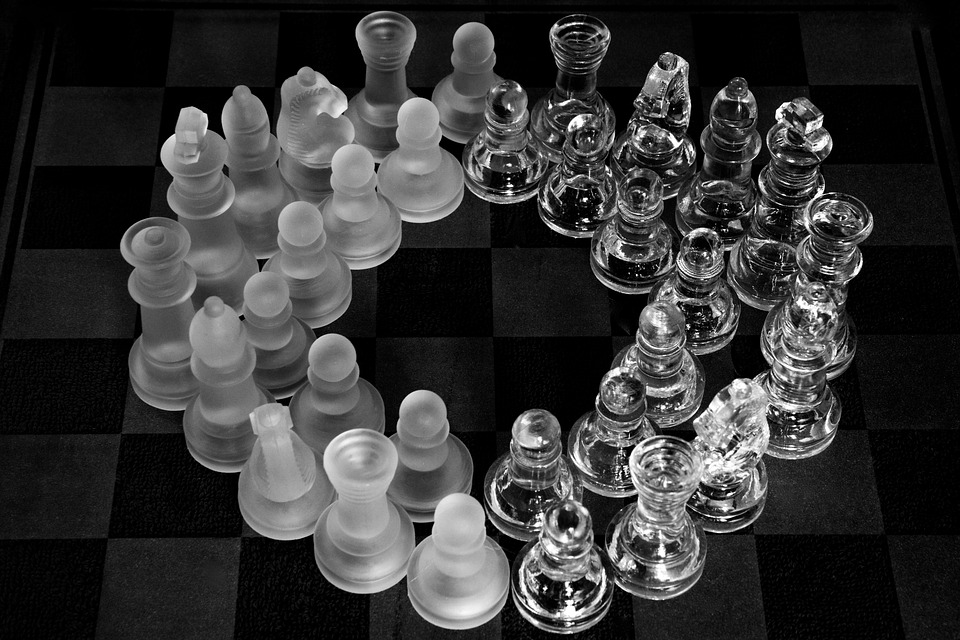
\includegraphics[width=\textwidth]{szklane_szachy.jpg}
		\captionsetup{font={up, footnotesize}}
    	\caption{Szklane szachy.}
		\label{rys6}
	\end{subfigure}
	\captionsetup{justification=raggedleft, font={it, footnotesize}}
	\caption*{\url{http://www.google.pl}} 
    \captionsetup{justification=justified, font={up, footnotesize}}
    \caption{Szachy i wszystko co z nimi związane. Takie ułożenie najbardziej pasuje do przedstawiania wykresów, bądź obrazków pochodzących z jednego źródła.}
    \label{rys7}
\end{figure}

\subsection{Tabele}

\begin{table}[H]
\caption{Przykład tabeli. Niestety szerokość kolumn należy ustawiać ręcznie.}
\centering
\footnotesize
\label{tab1}
\begin{tabular}{!{\color{sapphire}\vrule width 1pt}m{0.22\textwidth}!{\color{black}\vrule width 1pt}m{0.22\textwidth}!{\color{black}\vrule width 1pt}m{0.22\textwidth}!{\color{black}\vrule width 1pt}m{0.22\textwidth}!{\color{sapphire}\vrule width 1pt}}
	\arrayrulecolor{sapphire}\hline
	\Centering\bfseries Nazwa pierwiastka &
	\Centering\bfseries Symbol na tablicy Mendelejewa &
	\Centering\bfseries Liczba atomowa &
	\Centering\bfseries Nazwa pierwiastka pisana od tyłu \\
	\hline
	Hel & 
	\Centering He &
	\raggedleft 2 &
	Leh \\ 
	\arrayrulecolor{black}
	\hline
	Tlen & 
	\Centering O &
	\raggedleft 8 & 
	Nelt \\ 
	\hline
	Ołów & 
	\Centering Pb &
	\raggedleft 82 &
	Wóło \\
	\arrayrulecolor{sapphire}\hline
\end{tabular}
\captionsetup{justification=raggedleft, font={it, footnotesize}}
\caption*{\url{http://mm.pwn.pl/ency/jpg/583/1p/d93i6911.jpg}} 
\end{table}

\subsection{Kod źródłowy programu}

\begin{table}[H]
\caption{Kod źródłowy programu. Procedura czegośtam.}
\label{tab2}
\begin{lstlisting}[frame=single]  % Start your code-block

Actions(int nObjects, int radius, int width, int height)
{
	objects = new Ball[nObjects];
	connections = new int[nObjects][2];
	this.width = width;
	this.height = height;
		
	for(int i=0; i<objects.length; i++)
	{
		objects[i] = new Ball();
		objects[i].setX(randomWithRange(radius);
		objects[i].setY(randomWithRange(radius);
		objects[i].setRadius(radius);
		objects[i].setV(randomWithRange(1.0, 4.5));
		//objects[i].setV(4);
			
		connections[i][0] = -1;
		connections[i][1] = -1;
	}
		
	connectionsAssigned();
}
\end{lstlisting}
\end{table}

\newpage
\bibliographystyle{plain} % bibliography style
\bibliography{bibliography} % add bibliography


\end{document}
